\documentclass[12pt]{article}

\usepackage{graphicx}
\usepackage{paralist}
\usepackage{amsfonts}
\usepackage{amsmath}
\usepackage{hhline}
\usepackage{booktabs}
\usepackage{multirow}
\usepackage{multicol}
\usepackage{url}
\usepackage{tabto}

\oddsidemargin -10mm
\evensidemargin -10mm
\textwidth 160mm
\textheight 200mm
\renewcommand\baselinestretch{1.0}

\pagestyle {plain}
\pagenumbering{arabic}

\newcounter{stepnum}

%% Comments

\usepackage{color}

\newif\ifcomments\commentstrue

\ifcomments
\newcommand{\authornote}[3]{\textcolor{#1}{[#3 ---#2]}}
\newcommand{\todo}[1]{\textcolor{red}{[TODO: #1]}}
\else
\newcommand{\authornote}[3]{}
\newcommand{\todo}[1]{}
\fi

\newcommand{\wss}[1]{\authornote{blue}{SS}{#1}}

\title{Assignment 4, Design Specification}
\author{SFWRENG 2AA4}

\begin{document}

\maketitle
This Module Interface Specification (MIS) document contains modules, types and
methods for implementing the game \textit{2048}. At the start of each game, two random cells will be given number 2 or 4. Then the user can choose a move direction to move all the cells to that direction, if two cells have the same number, then they can be merged into a new cell with the number doubled. After that, the system will choose an empty cell (a cell with number 0 in implementation) to have a new number 2 or 4, with the probability of $90\%$ and $10\%$, respectively. Then the new round starts, the user chooses a move direction... The user will win when a cell with number 2048 appears in the board; otherwise, the game ends when the board is fulfilled with cells with number other than 0 and moving to any direction will not update the board. During the game, a score is updated by adding the number doubled to the current score when a merge happens.\\

Some special behaviors of these game are listed below:\\
\begin{itemize}
\item Merge can only happen between two old cells (the cells that are already on the board) during one movement. For example, if a row has the value $[2, 2, 2, 2]$ and the user chooses to move left, then the result is $[4, 4, 0, 0]$, rather than $[8, 0, 0, 0]$; if a row has the value $[2, 2, 4, 4]$ and the user chooses to move left, then the result is $[4, 8, 0, 0]$, rather than $[8, 4, 0, 0]$.
\item If the user choose to move to the direction that will not update the board (not change the numbers on the board), then no random 2 or 4 will be generated. This behavior is the same with the current online 2048 version, which in some way can avoid the unsatisfying cases caused by user's miss hitting.
\item Currently, the game can be played in the terminal. Enter one of "w", "s", "a", "d" to indicate move up, down, left, right, respectively. When you want to quit, just enter "exit", then you will quit the game and go back to terminal.
\end{itemize}

\begin{center}
  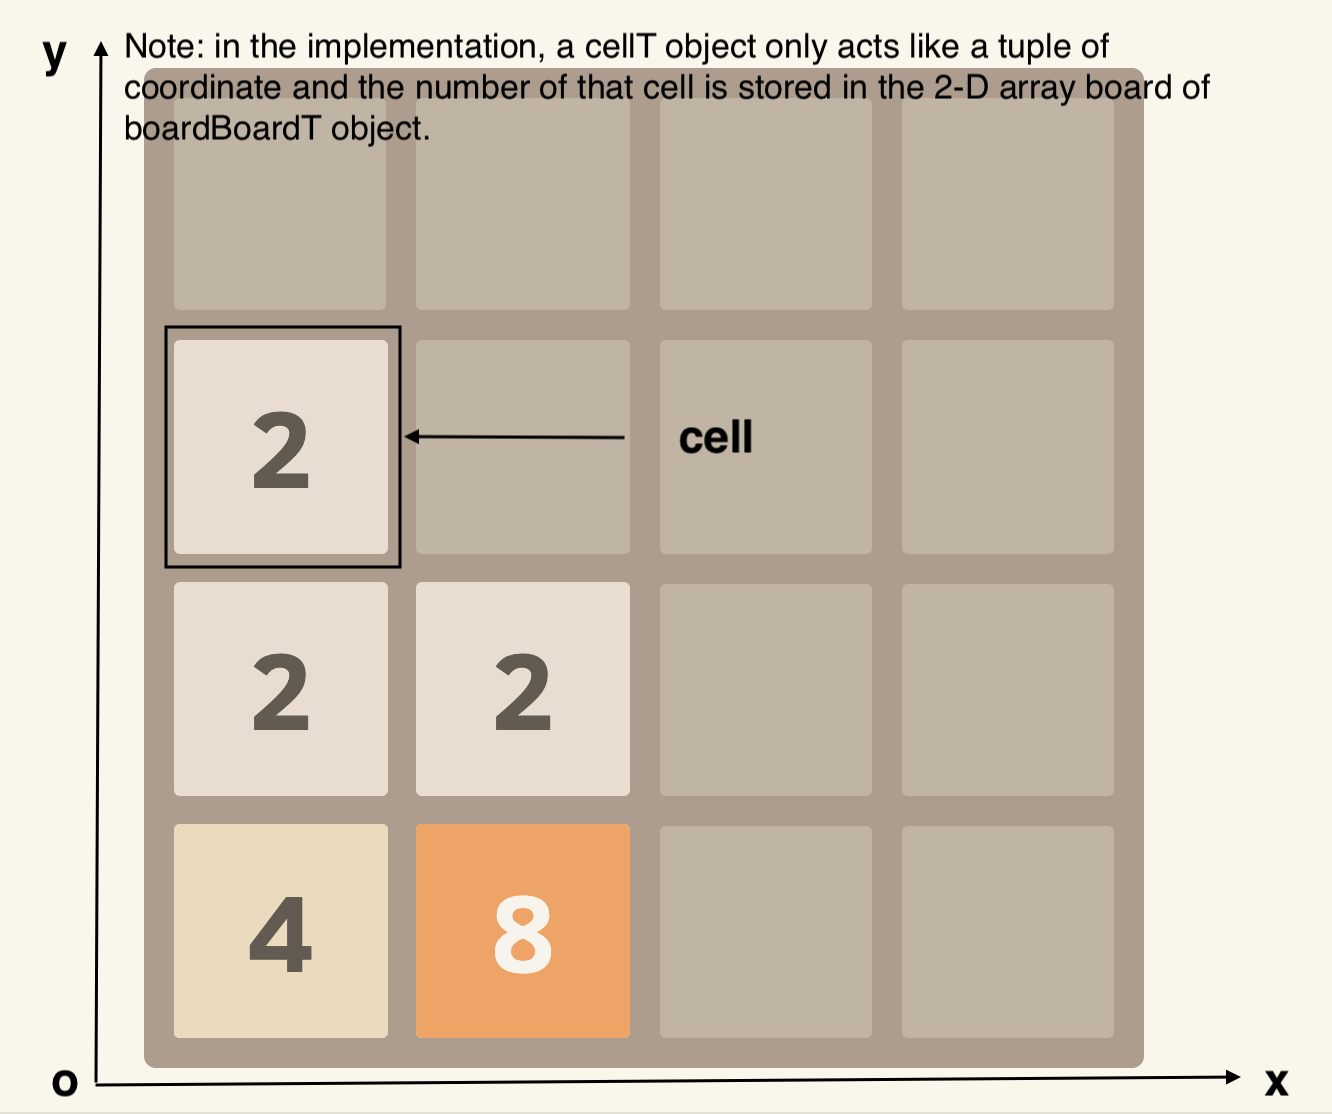
\includegraphics[width=0.8\textwidth]{data_structure.png}

  The above board visualization is from https://play2048.co/.
\end{center}

\newpage
\section*{How to Play : )}
In your terminal, cd to A4, enter \verb|make demo|. Then a prompt will be displayed. Enter any number for the game size (enter 4 or any invalid character for a `normal' game). To move the cells, enter one of "w"(up), "a"(left), "s"(down), "d"(right) and hit enter/return. During the game, if you want to quit, just enter "exit" and hit enter/return.\\

\noindent
Note: the main reason I choose to use "wasd" as the game control key is that the key mapping for arrows could raise some issues on different OSs.\\

\noindent
On the next page is a sample play trace for illustrating this process. Have fun : - )
\begin{center}
  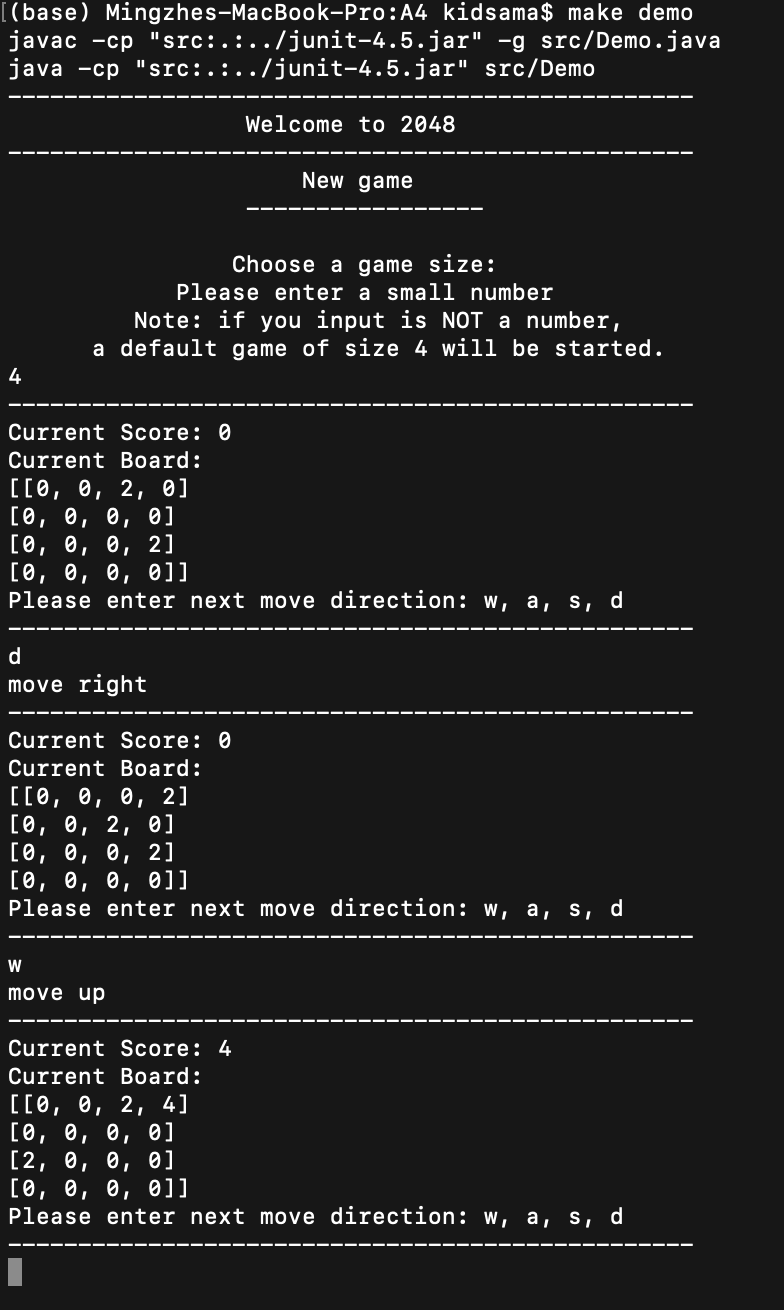
\includegraphics[width=0.8\textwidth]{hwp.png}
\end{center}


\newpage
\section*{Overview of the design}

This design applies Module View Specification (MVC) design pattern and Singleton design pattern. The MVC components are \textit{GameController} (controller module), \textit{BoardT} (model module), and \textit{UserInterface} (view module). Singleton pattern is specified and implemented for \textit{GameController} and \textit{UserInterface}.

\bigskip

%\noindent An UML diagram is provided below for visualizing the structure of this software architecture

%\includegraphics[width=0.9\textwidth]{UML_A4.png}

\noindent
The MVC design pattern is specified and implemented in the following way: the module \textit{BoardT}
stores the state of the game board and the status of the game. A view module \textit{UserInterface} can display
the state of the game board and game using a text-based graphics. The controller \textit{GameController}
is responsible for handling input actions. 

\bigskip

\noindent
For \textit{GameController} and \textit{UserInterface}, use the getInstance() method to obtain the abstract object.

\newpage

\subsection*{Likely Changes my design considers:}

\begin{itemize}
  \item Data structure used for storing the game board
  \item The visual representation of the game such as UI layout. 
  \item Change in peripheral devices for taking user input. 
  \item Change of the board size to adjust some variant versions of 2048.
\end{itemize}

\newpage

\section* {Cell ADT Module}

\subsection*{Template Module}

CellT

\subsection* {Uses}

None

\subsection* {Syntax}

\subsubsection* {Exported Constants}

None

\subsubsection* {Exported Types}

CellT = ?

\medskip

\subsubsection* {Exported Access Programs}

\begin{tabular}{| l | l | l | p{6cm} |}
\hline
\textbf{Routine name} & \textbf{In} & \textbf{Out} & \textbf{Exceptions}\\
\hline
CellT & $\mathbb{N}$, $\mathbb{N}$ & CellT & \\
\hline
getX & ~ & $\mathbb{N}$ & \\
\hline
getY & ~ & $\mathbb{N}$ & \\
\hline
\end{tabular}

\subsection* {Semantics}

\subsubsection* {State Variables}

x : $\mathbb{N}$\\
y : $\mathbb{N}$

\subsubsection* {State Invariant}

None

\subsubsection* {Access Routine Semantics}

new CellT(newX, newY):

\begin{itemize}
  \item output: out $:=$ self
  \item transition: x, y $:=$ newX, newY
\end{itemize}

\noindent getX():
\begin{itemize}
  \item output: out $:=$ x
\end{itemize}


\noindent getY():
\begin{itemize}
  \item output: out $:=$ y
\end{itemize}

\newpage

\section* {LinkedList ADT Module}

\subsection*{Template Module}

LinkedList

\subsection* {Uses}

None

\subsection* {Syntax}

\subsubsection* {Exported Constants}

None

\subsubsection* {Exported Types}

LinkedList = ?

\medskip

\subsubsection* {Exported Access Programs}

\begin{tabular}{| l | l | l | p{6cm} |}
\hline
\textbf{Routine name} & \textbf{In} & \textbf{Out} & \textbf{Exceptions}\\
\hline
LinkedList & ~ & LinkedList &  LinkedListERROR\\
\hline
add & $\mathbb{N}$ & ~ &  addERROR\\
\hline
pop & ~ & $\mathbb{N}$ &  popERROR\\
\hline
peek & ~ & $\mathbb{N}$ &  peekERROR\\
\hline
addAll & LinkedList & ~ &  addAllERROR\\
\hline
isEmpty & ~ & $\mathbb{B}$ & isEmptyERROR\\
\hline
size & ~ & $\mathbb{N}$ &  sizeERROR\\
\hline
\end{tabular}

\subsection*{Consideration}
The \verb|LinkedList| class is already in the java library. The above is only an list of the methods used in this design.

\newpage

\section* {Board ADT Module}

\subsection*{Template Module}

BoardT

\subsection* {Uses}

CellT, LinkedList, MoveDirection

\subsection* {Syntax}

\subsubsection* {Exported Types}

BoardT = ?

\subsubsection* {Exported Constant}

None

\subsubsection* {Exported Access Programs}

\begin{tabular}{| l | l | l | l |}
\hline
\textbf{Routine name} & \textbf{In} & \textbf{Out} & \textbf{Exceptions}\\
\hline
BoardT & $\mathbb{N}$ & BoardT & \\
\hline
setBoard & seq of (seq of $\mathbb{N}$) & ~ & \\
\hline
setScore & $\mathbb{N}$ & ~ & \\
\hline
getBoard & ~ & seq of (seq of $\mathbb{N}$) & \\
\hline
getScore & ~ & $\mathbb{N}$ & \\
\hline
getSize & ~ & $\mathbb{N}$ & \\
\hline
getEmptyCells & ~ & seq of CellT & \\
\hline
isGen24Flag & ~ & $\mathbb{B}$ & \\
\hline
moveDown & ~ & seq of (seq of $\mathbb{N}$) & \\ % direction based on user's view
\hline
down & ~ & ~ & \\
\hline
up & ~ & ~ & \\
\hline
left & ~ & ~ & \\
\hline
right & ~ & ~ & \\
\hline
move & MoveDirection & ~ & \\
\hline
genRand2Or4 & ~ & ~ & \\
\hline
isWin & ~ & $\mathbb{B}$ & \\
\hline
isLoose & ~ & $\mathbb{B}$ & \\
\hline




\end{tabular}

\noindent
\# Note:  \verb|getEmptyCells| and \verb|getEmptyCells| both return an arraylist.

\subsection* {Semantics}

\subsubsection* {State Variables}

board: seq of (seq of $\mathbb{N}$) \# the length of this 2d array is specified by the constructor.\\
score: $\mathbb{N}$ \\
gen24Flag: $\mathbb{B}$ \\

\subsubsection* {State Invariant}

None

\subsubsection* {Assumptions}

\begin{itemize}
  \item The constructor BoardT is called for each object instance before any other access routine 
  is called for that object. 
  \item Assume there is a random function that generates a random value beteern 0 and 1.
\end{itemize}

\subsubsection* {Design decision}

The coordinates of the board is stored in a 2D sequence. The coordinates used for retriving the cell is different
from the coordinate entered by the user. When the user refers to row 0 and column 0 cell 
on their screen, that cell is actually stored in board[0][3]. Thus, board[0][0] is located at bottom left corner of the UI 
and board[3][3] is located at top right corner of the UI.

\begin{center}
  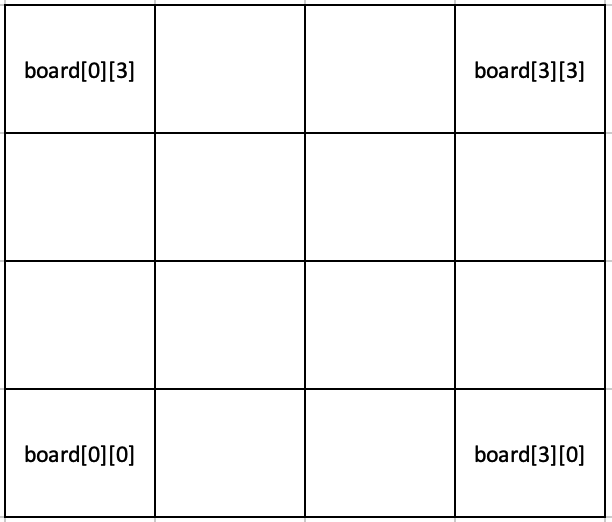
\includegraphics[width=0.6\textwidth]{board.png} \\
  In the above illustration, the number in (0,0) of the UI is stored in board[0][3].
\end{center}

\begin{itemize}
  \item The main reason I store the board in this way is for the ease of cell merge process. It is easier to perform move down operation if those cells are in the same row. Since each row of the board is represented as a column on the UI. The linkedlist operations like pop, peak and add can be naturally used in a row to simulate a drop down on the UI.
\end{itemize}

\subsubsection* {Access Routine Semantics}

BoardT():
\begin{itemize}
\item transition: \\
      board $:=$ 
      $\langle \begin{array}{c}
      \langle 0, ... ... , 0 \rangle\\
      \langle 0, ... ... , 0 \rangle\\
      ... ...\\
	 \langle 0, ... ... , 0 \rangle\\
      \end{array} \rangle$ \\ \\
      score, gen24Flag $=$ 0, true
\item output: $out := \mathit{self}$
\item exception: None
\end{itemize}

\noindent setBoard(b):
\begin{itemize}
\item transition: board $:=$ b
\item output: None
\item exception: None
\end{itemize}

\noindent setScore(s):
\begin{itemize}
\item transition: score $:=$ s
\item output: None
\item exception: None
\end{itemize}

\noindent getBoard():
\begin{itemize}
\item transition: none
\item output: $out :=$ $\langle \forall x, y : \mathbb{N} \mid 0 \leq x,y \leq |board| - 1 : board[x][y] \rangle$
\item exception: None
\end{itemize}

\noindent getScore():
\begin{itemize}
\item transition: none
\item output: $out :=$ score
\item exception: None
\end{itemize}

\noindent getSize():
\begin{itemize}
\item transition: none
\item output: $out :=$ board.length
\item exception: None
\end{itemize}

\noindent getEmptyCells():
\begin{itemize}
\item transition: none
\item output: $out :=$ $\langle \forall i, j : \mathbb{N} \mid board[i][j] = 0 : CellT(i, j) \rangle$
\item exception: None
\end{itemize}

\noindent isGen24Flag():
\begin{itemize}
\item transition: none
\item output: $out :=$ gen24Flag
\item exception: None
\end{itemize}

% need to be imroved
\noindent moveDown():
\begin{itemize}
\item transition: \# procedural specification\\\\
newBoard = new Seq$[|board|]$ of (Seq$[|board|]$ of $\mathbb{N}$)\\
for x in $\langle 0, 1, ..., |board|-1 \rangle$\\
\tabto{0.5cm} curColum = new LinkedList()\\
\tabto{0.5cm} for y in $\langle 0, 1, ..., |board|-1 \rangle$\\
\tabto{1.0cm} if board$[x][y] > 0$\\
\tabto{1.5cm} curColum.add(board$[x][y]$)\\
\tabto{0.5cm} newColum = new LinkedList()\\
\tabto{0.5cm} while curColum.size() $\geq$ 2\\
\tabto{1.0cm} firstNum = curColum.pop()\\
\tabto{1.0cm} secondNum = curColum.peek()\\
\tabto{1.0cm} if firstNum = secondNum\\
\tabto{1.5cm} newColum.add(firstNum $*$ 2)\\
\tabto{1.5cm} score = score + firstNum $*$ 2
\tabto{1.5cm} curColum.pop()\\
\tabto{1.0cm} else\\
\tabto{1.5cm} newColum.add(firstNum)\\
\tabto{0.5cm} newColum.addAll(curColum)\\
\tabto{0.5cm} newBoard[x] = new Seq$[|board|]$ of $\mathbb{N}$\\
\tabto{0.5cm} for y in $\langle 0, 1, ..., |board|-1 \rangle$\\
\tabto{1.0cm} if newColum.isEmpty()\\
\tabto{1.5cm} newBoard[x][y] = 0\\
\tabto{1.0cm} else\\
\tabto{1.5cm} newBoard[x][y] = newColum.pop()


\item output: $out :=$ newBoard
\item exception: None
\end{itemize}

\noindent down():
\begin{itemize}
\item transition: \# procedural specification\\\\
board = moveDown()
\item output: None
\item exception: None
\end{itemize}
~\noindent \# moveDown will implicitly update the gen24Flag and score field as listed above.\\

\noindent up():
\begin{itemize}
\item transition: \# procedural specification\\\\
board = mirrorLeftRight(board)\\
board = mirrorLeftRight(moveDown())
\item output: None
\item exception: None
\end{itemize}
~\noindent \# moveDown will implicitly update the gen24Flag and score field as listed above.\\

\noindent left():
\begin{itemize}
\item transition: \# procedural specification\\\\
board = transpose(board)\\
board = transpose(moveDown())
\item output: None
\item exception: None
\end{itemize}
~\noindent \# moveDown will implicitly update the gen24Flag and score field as listed above.\\

\noindent right():
\begin{itemize}
\item transition: \# procedural specification\\\\
board = transpose(board)\\
board = mirrorLeftRight(board)\\
board = transpose(mirrorLeftRight(moveDown()))
\item output: None
\item exception: None
\end{itemize}
~\noindent \# moveDown will implicitly update the gen24Flag and score field as listed above.\\

\noindent move(m):
\begin{itemize}
\item transition: \# procedural specification\\\\
(m = moveDirection.UP $\Rightarrow$ up() $\mid$ m = moveDirection.DOWN $\Rightarrow$ down() $\mid$ m = moveDirection.LEFT $\Rightarrow$ left() $\mid$ m = moveDirection.RIGHT $\Rightarrow$ right())
\item output: None
\item exception: None
\end{itemize}
~\noindent \# moveDown will implicitly update the gen24Flag and score field as listed above.\\

\noindent genRand2Or4():
\begin{itemize}
\item transition: \# procedural specification\\\\
Randomly select a cell from all cells in getEmptyCells(), then update the board[cell.getX()][cell.getY()] to 2 or 4, whose occurrence probability is 90\% and 20\%, respectively.
\item output: None
\item exception: None
\end{itemize}

\noindent isWin():
\begin{itemize}
\item transition: None
\item output: out $:=$ $\exists(x, y : \mathbb{N} \mid 0 \leq x, y \leq |board| - 1  : board[x][y] = 2048)$
\item exception: None
\end{itemize}

\noindent isLoose():
\begin{itemize}
\item transition: None
\item output: $out :=$ compareTwoInt2DArr(oldBoard, newBoard1) $\land$ compareTwoInt2DArr(oldBoard, newBoard2) $\land$ compareTwoInt2DArr(oldBoard, newBoard3) $\land$ compareTwoInt2DArr(oldBoard, newBoard4), \\
where oldBoard is the current board state, newBoard1, newBoard2, newBoard3 and newBoard4 are the new board states after calling up(), down(), left(), and right(), respectively.
\item exception: None
\end{itemize}

\subsection*{Local Functions}
\noindent transpose: Seq of (Seq of $ \mathbb{N}$) $\rightarrow$ Seq of (Seq of $\mathbb{N}$)\\
\noindent transpose(inputArr) $\equiv$\\
$\langle \begin{array}{c}
      \langle a_{00}, a_{10}, ... ... , a_{n0} \rangle\\
      \langle a_{01}, a_{11}, ... ... , a_{n1} \rangle\\
      ... ...\\
	 \langle a_{0n}, a_{1n}, ... ... , a_{nn} \rangle\\
      \end{array} \rangle$,\\\\
when inputArr = \\\\
$\langle \begin{array}{c}
      \langle a_{00}, a_{01}, ... ... , a_{0n} \rangle\\
      \langle a_{10}, a_{11}, ... ... , a_{1n} \rangle\\
      ... ...\\
	 \langle a_{n0}, a_{n1}, ... ... , a_{nn} \rangle\\
      \end{array} \rangle$,\\\\
where n = $|inputArr|$.\\

\medskip

\noindent mirrorLeftRight: Seq of (Seq of $ \mathbb{N}$) $\rightarrow$ Seq of (Seq of $\mathbb{N}$)\\
\noindent mirrorLeftRight(inputArr) $\equiv$\\
$\langle \begin{array}{c}
      \langle a_{0n},  ... ... , a_{01}, a_{00} \rangle\\
      \langle a_{1n},  ... ... , a_{11}, a_{10} \rangle\\
      ... ...\\
	 \langle a_{nn},  ... ... , a_{n1}, a_{n0} \rangle\\
      \end{array} \rangle$,\\\\
when inputArr = \\\\
$\langle \begin{array}{c}
      \langle a_{00}, a_{01}, ... ... , a_{0n} \rangle\\
      \langle a_{10}, a_{11}, ... ... , a_{1n} \rangle\\
      ... ...\\
	 \langle a_{n0}, a_{n1}, ... ... , a_{nn} \rangle\\
      \end{array} \rangle$,\\\\
where n = $|inputArr|$.\\

\medskip

\noindent compareTwoInt2DArr: Seq of (Seq of $ \mathbb{N}$) $\times$ Seq of (Seq of $\mathbb{N}$) $\rightarrow$ $\mathbb{B}$\\
\noindent compareTwoInt2DArr(arr1, arr2) $\equiv$ 
$(|arr1| \neq |arr2| \Rightarrow False \mid (\forall x : \mathbb{N} \mid 0 \leq x \leq |arr1| - 1 :|arr1[x]| \neq |arr2[x]|) \Rightarrow False \mid (\forall x, y : \mathbb{N} \mid x, y \in [0, .., |arr1| - 1] : arr1[x][y] = arr2[x][y]) \Rightarrow True)$.

\newpage

\section* {UserInterface Module}

\subsection* {UserInterface Module}

\subsection* {Uses}

None

\subsection* {Syntax}

\subsubsection* {Exported Types}

None

\subsubsection* {Exported Constants}

None

\subsubsection* {Exported Access Programs}

\begin{tabular}{| l | l | l | p{6cm} |}
\hline
\textbf{Routine name} & \textbf{In} & \textbf{Out} & \textbf{Exceptions}\\
\hline
getInstance & ~ & UserInterface &  \\
\hline
printBoard & Seq of (Seq of $\mathbb{N}$), $\mathbb{N}$ & ~ & \\
\hline
printWelcomeMessage & ~ & ~ & \\
\hline
printGameSizePrompt & ~ & ~ & \\
\hline
printWinningMessage & ~ & ~ & \\
\hline
printLosingMessage & $\mathbb{N}$ & ~ & \\
\hline
printEndingMessage & ~ & ~ & \\
\hline
\end{tabular}

\subsection* {Semantics}

\subsection*{Environment Variables}

window: A portion of computer screen to display the game and messages

\subsubsection* {State Variables}

visual: UserInterface

\subsubsection* {State Invariant}

None

\subsubsection* {Assumptions}

\begin{itemize}
\item The UserInterface constructor is called for each object instance before any
other access routine is called for that object.  The constructor can only be
called once.
\end{itemize}

\subsubsection* {Access Routine Semantics}

\noindent getInstance():
\begin{itemize}
  \item transition: visual $:=$ (visual = null $\Rightarrow$ new UserInterface())
  \item output: \textit{self}
  \item exception: None
\end{itemize}

\noindent printWelcomeMessage():
\begin{itemize}
\item transition: window $:=$ Displays a welcome message when user first enter the game.
\end{itemize}

\noindent printBoard($board$, $score$):
\begin{itemize}
\item transition: window $:=$ Draws the game board onto the screen. Each cell of the board
                  is accessed by traversing the 2D array board of $BoardT$. The board[x][y] is displayed 
                  in a way such that x is increasing from the left of the screen to the right,
                  and y value is increasing from the bottom to the top of the screen. For example,
                  board[0][0] is displayed at the bottom left corner and board[4][4] is displayed 
                  at top-right corner. 
\end{itemize}

\noindent printGameSizePrompt():
\begin{itemize}
\item transition: window $:=$ Window appends a prompt message asking the user to enter a number as the game board size.
\end{itemize}

\noindent printWinningMessage():
\begin{itemize}
\item transition: window $:=$ Prints a congratulation message after the the user wins.
\end{itemize}

\noindent printLosingMessage($score$):
\begin{itemize}
\item transition: window $:=$ Prints a message showing the final score after the the user looses.
\end{itemize}

\noindent printEndingMessage():
\begin{itemize}
\item transition: Prints a ending message after the the user either wins or looses.
\end{itemize}

\subsubsection*{Local Function:}

UserInterface: void $\rightarrow$ UserInterface \\
UserInterface() $\equiv$ new UserInterface()

\newpage

\section* {GameController Module}

\subsection* {GameController Module}

\subsection* {Uses}

BoardT, UserInterface

\subsection* {Syntax}

\subsubsection* {Exported Types}

None

\subsubsection* {Exported Constants}

None

\subsubsection* {Exported Access Programs}

\begin{tabular}{| l | l | l | p{4.7cm} |}
\hline
\textbf{Routine name} & \textbf{In} & \textbf{Out} & \textbf{Exceptions}\\
\hline
getInstance & BoardT, UserInterface & GameController & ~ \\
\hline
initializeGame & $\mathbb{N}$ & ~ & ~\\
\hline
readGameSizeInput& ~ & $\mathbb{N}$ & ~ \\
\hline
displayWelcomeMessage& ~ & ~ & ~ \\
\hline
displayBoard& ~ & ~ & ~ \\
\hline
displayWinningMessage& ~ & ~ & ~ \\
\hline
displayLosingMessage& ~ & ~ & ~ \\
\hline
displayEnding& ~ & ~ & ~ \\
\hline
displayGameSizePrompt& ~ & ~ & ~ \\
\hline
readUserMove & ~ & ~ & InputMismatchException \\
\hline
runGame & ~ & ~ & ~ \\
\hline
\end{tabular}

\subsection* {Semantics}

\subsection*{Environment Variables}

keyboard: Scanner(System.in) \qquad \textit{// reading inputs from keyboard}

\subsubsection* {State Variables}

model: BoardT \\
view: UserInterface \\
controller: GameController

\subsubsection* {State Invariant}

None

\subsubsection* {Assumptions}

\begin{itemize}
  \item The GameController constructor is called for each object instance before any
  other access routine is called for that object.  The constructor can only be
  called once.
  \item Assume that model and view instances are already initialized before calling GameController
        constructor
\end{itemize}

\subsubsection* {Access Routine Semantics}

getInstance($m$, $v$):
\begin{itemize}
  \item transition: controller $:=$ (controller = null $\Rightarrow$ new GameController ($m, v$))
  \item output: \textit{self}
  \item exception: None
\end{itemize}

\noindent initializeGame($size$):
\begin{itemize}
  \item transition: model $:=$ $new BoardT(size)$
  \item output: None
  \item exception: None
\end{itemize}

\noindent readGameSizeInput():
\begin{itemize}
  \item output: $out :=$ (input is a integer, entered from the keyboard by the User $\Rightarrow$ input $\mid$ 4)
  \item exception: None
\end{itemize}

\noindent displayWelcomeMessage():
\begin{itemize}
  \item transition: view $:=$ view.printWelcomeMessage()
\end{itemize}

\noindent displayBoard():
\begin{itemize}
  \item transition: view $:=$ view.printBoard($model.getBoard()$, $model.getScore()$)
\end{itemize}

\noindent displayWinningMessage():
\begin{itemize}
  \item transition: view $:=$ view.printWinningMessage()
\end{itemize}

\noindent displayLosingMessage():
\begin{itemize}
  \item transition: view $:=$ view.printWinningMessage($model.getScore()$)
\end{itemize}

\noindent displayEndingMessage():
\begin{itemize}
  \item transition: view $:=$ view.printEndingMessage()
\end{itemize}

\noindent displayGameSizePrompt():
\begin{itemize}
  \item transition: view $:=$ view.printGameSizePrompt()
\end{itemize}

\noindent readUserMove():
\begin{itemize}
  \item transition: None
  \item output: out $:=$ $((input = $`w'$ \Rightarrow MoveDirection.UP) \mid  (input = $`a'$ \Rightarrow MoveDirection.LEFT) \mid  (input = $`s'$ \Rightarrow MoveDirection.DOWN) \mid  (input = $`d'$ \Rightarrow MoveDirection.RIGHT))$ $\mid  (input = $`exit'$ \Rightarrow System.exit(0)))$, where input $: char$, entered from the keyboard by the User.
  \item exception: exc $:=$ ((input $\neq$ $`w'$ $\land$ input $\neq$ $`a'$ $\land$ input $\neq$ $`s'$ $\land$ input $\neq$ $`d'$) $\Rightarrow$ InputMismatchException).
\end{itemize}

\noindent runGame():
\begin{itemize}
  \item transition: operational method for running the game. The game will start with a welcome message, next
                    asking the user to enter a game board size (the default size is 4), then display the board and let the user to play the game. 
                    Eventually, when the game ends, prompt a winning or loosing message.
  \item output: None
\end{itemize}

\subsubsection*{Local Function:}

GameController: BoardT $\times$ UserInterface $\rightarrow$ GameController \\
GameController($model, view$) $\equiv$ new GameController($model, view$)

\newpage

\section*{Critique of Design}
\begin{itemize}
\item For all of the modules, the \verb|BoardT| is designed to be an ADT, because a board should be updated during the game; while \verb|GameController| and \verb|UserInterface| are designed to be an abstract object using an singleton design strategy, which I think can help avoid odd behaviors in the game running time and save necessary memory space.
\item The \verb|CellT| module is only like a typo class that stores the coordinate information, while the number of each cell is still stored in the board field of \verb|BoardT|. This design may seem no
\textbf{essential}, but it can be used to support other game variants or the later GUI work.
\item By designing an enum class \verb|MoveDirection|, the system can deal with all user's movement during the game, instead of deal with Strings that can easily raise exceptions.
\item The 2D array state variable of BoardT is also named board, whose naming convention may seem not \textbf{consistent}. But as many online resources and previous assignment use this naming, I think follow this convention can make my modules more understandable.
\item This MIS is \textbf{general} because instead of only supporting the classical 2048, user can also specify a new board size, which can make the game more fun. In addition, the \verb|CellT| is here to deal with future changes like a GUI requirement.
\item The \verb|moveDown| method in \verb|BoardT| violates the \textbf{minimality} principle, because it uses an algorithm to compute the entire board after move down and in the meantime updates the score. I think its unminimal cannot be avoided in the case that we want the game running more efficiently.
\item This design is \textbf{high cohesion and low coupling} mostly because the using of MVC design strategy. The \verb|GameController| updates the \verb|BoardT| and uses \verb|UserInterface| to display current state.
\item The \textbf{information hiding} is good. By using \verb|GameController| in the Demo, we can ignore all other unnecessary implementation details in other methods, which make the software easy to use.\
\item Did not build any test cases for testing the controller module since the implementation of the controller's access methods uses methods from the model and view. The test cases for the model are in \verb|TestBoardT.java|.
\item In this design, I also use a singleton design pattern in both \verb|GameController| and \verb|UserInterface|, for which we can only generate one instance. During the developing process, using static methods and variables usually cause some warnings about the method or variables to need to be accessed statically. Using singleton pattern eliminates all these problems, making a smoother development.
\end{itemize}

\newpage
\section*{Answers to Questions:}
\subsection*{Q1}

\begin{figure}[hbt!]
  \centering
  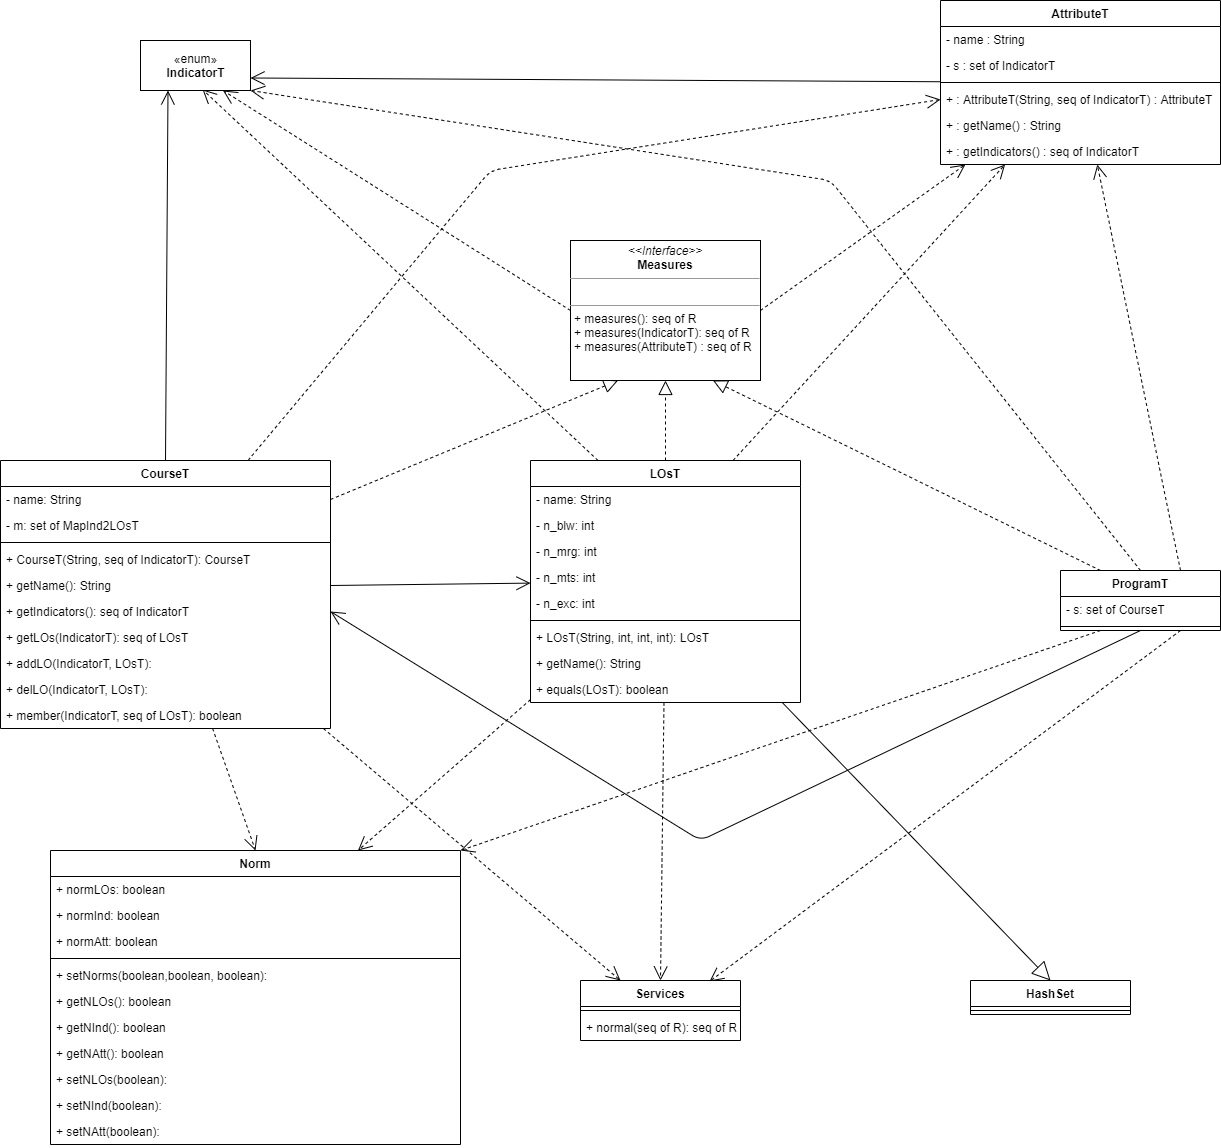
\includegraphics[width=1.0\textwidth]{UML.png}
\end{figure}

\newpage
\subsection*{Q2}
\begin{figure}[hbt!]
  \centering
  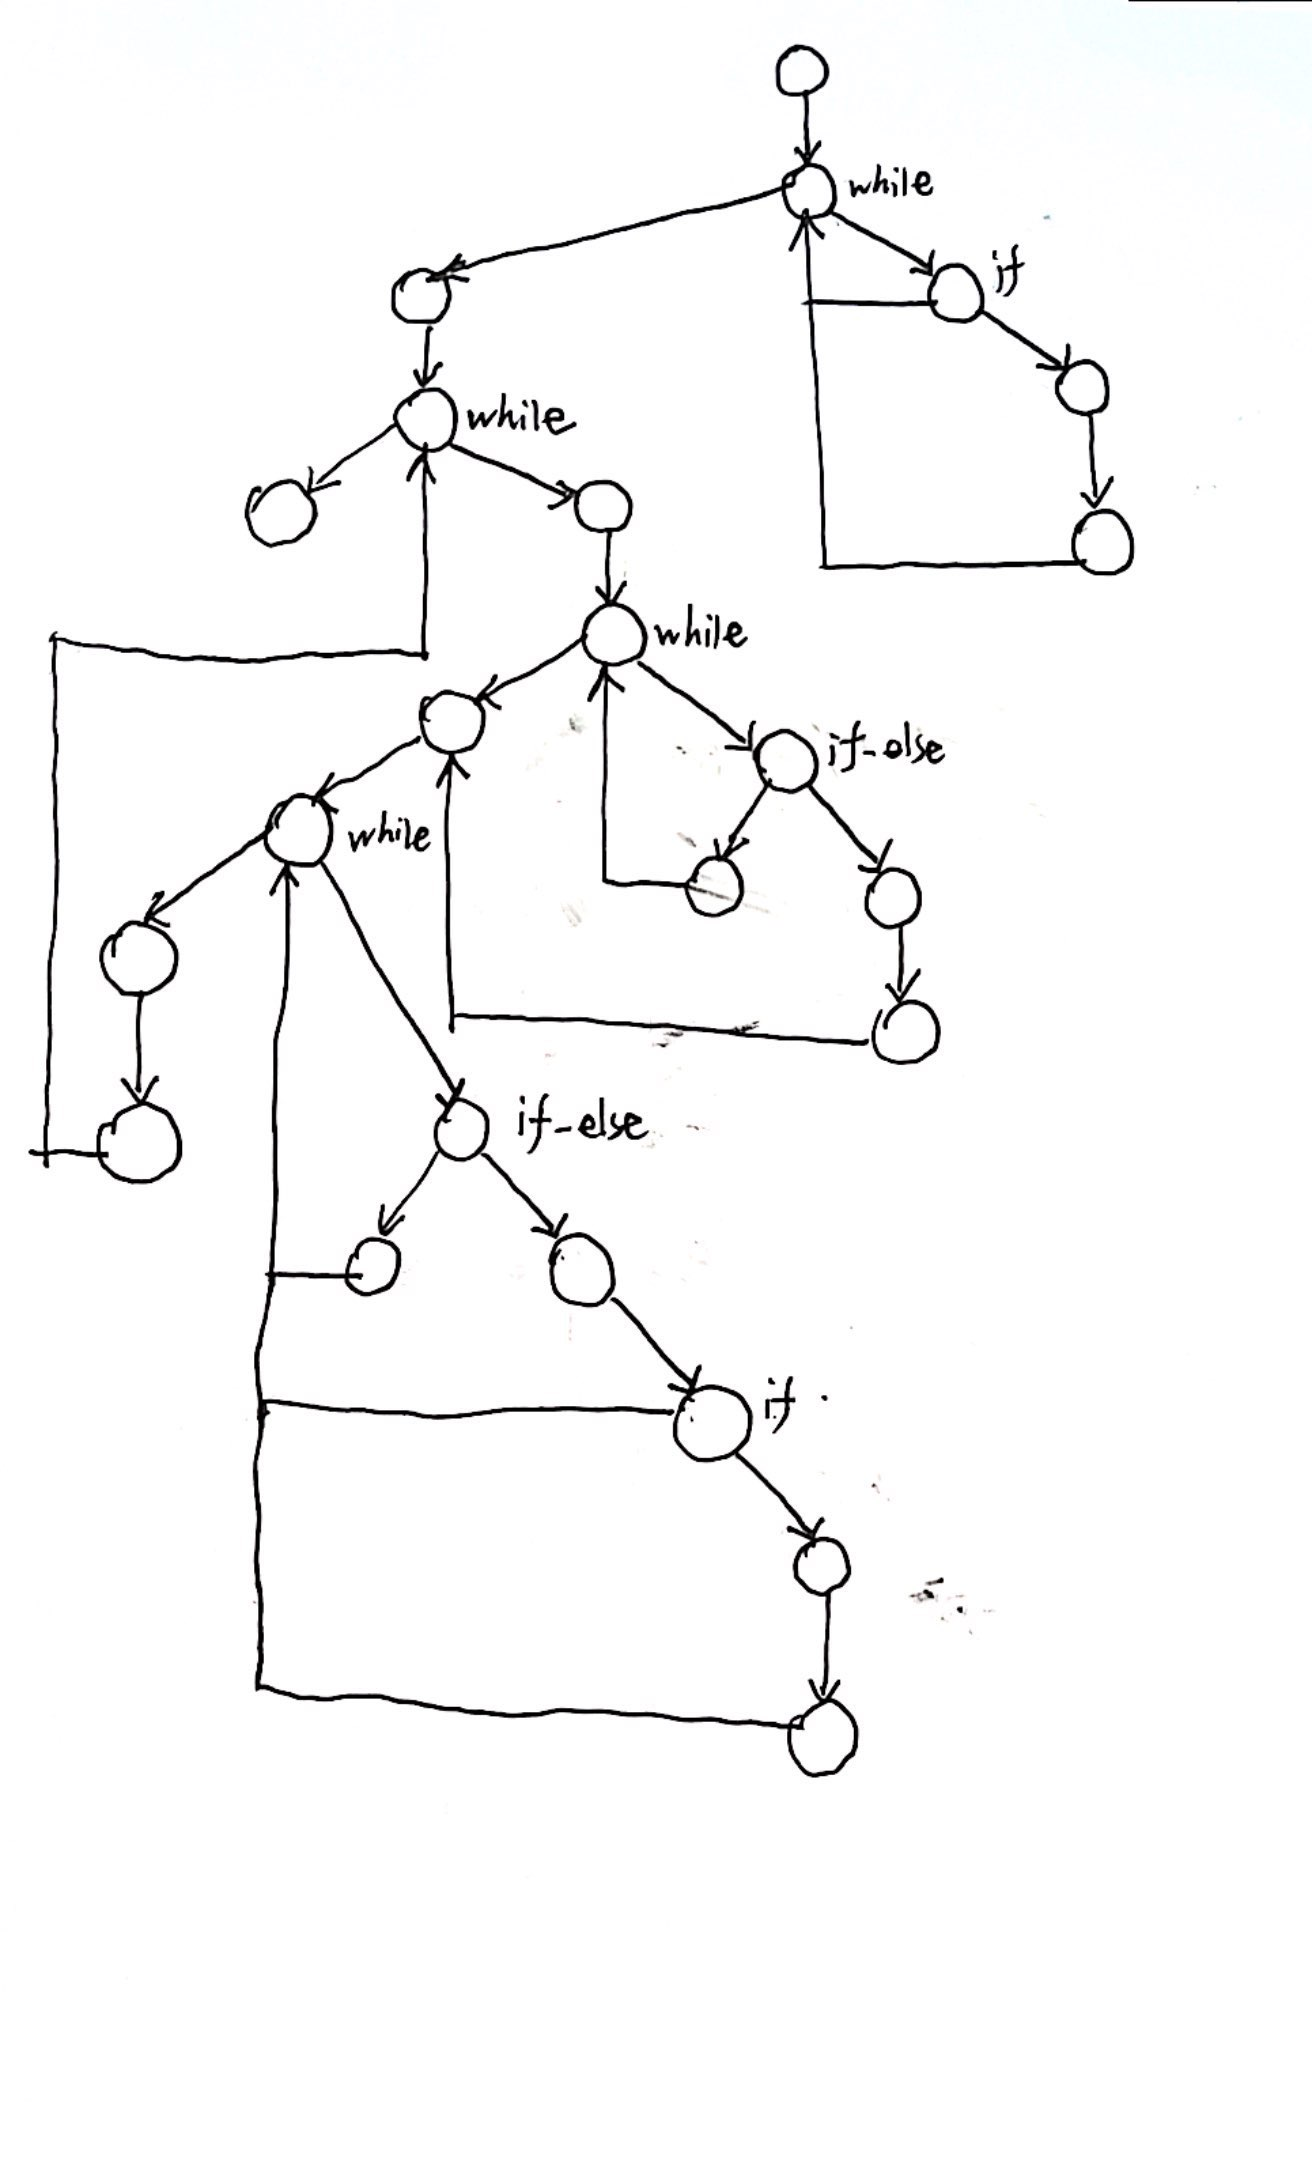
\includegraphics[width=0.7\textwidth]{control_flow.jpg}
\end{figure}

\end {document}